\chapter{Implementation des BruteForce-Algorithmus}
\label{implementation}
In diesem Kapitel wird die Konzeption des Brute Force-Angriffs beschrieben. Auf Basis der beschriebenen Konzeption soll im Anschluss die Implementation erfolgen können. 



\section{Architektur}
In diesem Kapitel wird die geplante Architektur des verteilten Systems beschrieben. \\
Generell wird die Kommunikation nachrichtenbasiert umgesetzt. Dies bedeutet, dass die Komponenten des verteilten Systems kommunizieren, indem sie sich Nachrichten übermitteln können. Die Steuerung der Kommunikation wird primär von den als Master (siehe Glossar) ausgewählten Komponenten umgesetzt. Als Provider wird ein angepasster Webserver eingesetzt, die Verbindung der einzelnen Komponenten zueinander geschieht über WebSockets. Der Webserver basiert auf dem Javascript-Framework Node.js. \\
Details der nachrichtenbasierten Kommunikation werden nun in den folgenden Kapiteln beschrieben. 


\subsection{Nachrichtenstruktur}
Da unsere Implementation auf einer nachrichtenbasierten Kommunikation basieren wird, ist der Entwurf eigener Nachrichtenstrukturen notwendig. Die Nachrichtenstrukturen übertragen alle projektrelevanten Informationen zwischen den Mastern und den Workern. Zur Strukturierung fiel die Wahl auf das Nachrichtenaustauschformat \enquote{JavaScript Object Notation} oder kurz \emph{JSON}, da dieses Format sehr leichtgewichtig und einfach anpassbar ist. \\
Nachfolgend werden die entwickelten Nachrichtenstrukturen und deren Inhalt detailliert beschrieben. Die Nachrichten werden in drei Kategorien unterteilt: Nachrichten zum Worker, Nachrichten zum Master und allgemeine Nachrichten.

\subsubsection{Nachrichten zum Worker}
Hier werden die Strukturen beschrieben, welche vom steuernden Rechner (Master) zu einem der Worker gesendet werden.\\

\texttt{SetupAndConfig}
\begin{lstlisting}[basicstyle=\ttfamily,numbers=left,numberstyle=\footnotesize\ttfamily,backgroundcolor=\color{sourcegray}]
{
  "status" : "setupConfig",
  "value" : {
    "algorithm" : "#HASH_ID",
    "target" : "#TARGET_HASH", 
    "worker_id" : "#WORKER_ID"
  }
}
\end{lstlisting}
Ein im Cluster neu hinzugefügter Worker erhält seine Konfigurationsparameter, damit dieser mit dem Berechnen beginnen kann. 
Der Wert \textbf{algorithm} übergibt die ID des Hash-Algorithmus, welcher in der aktuellen Passwortberechnung benutzt wird. \textbf{Target} übermittelt den Hash des Zielpasswortes. Anhand des Hashes kann ein Worker bestimmen, ob das Zielpasswort berechnet wurde. Die \textbf{workerID} ist eine vom Master vergebene, fortlaufende Nummer und dient der Identifizierung der Worker.\\

\texttt{getWork}
\begin{lstlisting}[basicstyle=\ttfamily,numbers=left,numberstyle=\footnotesize\ttfamily,backgroundcolor=\color{sourcegray}]
{
	"status" : "newWorkBlog",
  	"value" : "#NEW_HASH(ES)"
}
\end{lstlisting}
Diese Nachricht übermittelt dem Worker eine Anzahl neuer Passwörter, von denen dieser die Hashes berechnen wird.


\subsubsection{Nachrichten zum Master}
Folgende Nachrichten werden von den Workern an die Master gesendet. \\

\texttt{newClientRegistration}
\begin{lstlisting}[basicstyle=\ttfamily,numbers=left,numberstyle=\footnotesize\ttfamily,backgroundcolor=\color{sourcegray}]
{
  "status" : "newClientRegistration",
  "value" : {
    "worker" : "#WORKER_ID"
  }
}
\end{lstlisting}
Der Worker beantragt eine ID, um sich im Cluster identifizieren zu können.\\

\texttt{hitTargetHash}
\begin{lstlisting}[basicstyle=\ttfamily,numbers=left,numberstyle=\footnotesize\ttfamily,backgroundcolor=\color{sourcegray}]
{
  "status" : "hitTargetHash",
  "value" : {
    "hash" : "#HASH_VALUE",
    "password" : "#PASSWORD"
    "time_needed" : "#TIME"
  }
}\end{lstlisting}
Diese Nachricht wird vom Worker versendet, wenn der berechnete Hash dem Zielhash entspricht und somit das Passwort berechnet wurde. Es werden der berechnete Hash und das zugehörige Passwort übertragen. Zudem wird die Zeit, die die Berechnung in Anspruch genommen hat, übertragen. Die Zeit kann für spätere Erweiterungen des Projekts genutzt werden, beispielsweise zum Vergleich verschiedener Hash-Algorithmen.\\

\texttt{finishedWork}
\begin{lstlisting}[basicstyle=\ttfamily,numbers=left,numberstyle=\footnotesize\ttfamily,backgroundcolor=\color{sourcegray}]
{
  "status" : "finishedWork",
  "value" : "#WORKER_ID"
}
\end{lstlisting}
Mit dieser Nachricht teilt der Worker mit, dass alle möglichen Passworte des aktuellen Arbeitspakets berechnet worden sind. Falls bei der Berechnung der Zielhash bzw. das Zielpasswort berechnet worden ist, wird zusätzlich die Nachricht \enquote{finishedWork} versandt. Ansonsten erhält der Worker ein neues Arbeitspaket aus dem Nachrichtenstrom. \\

\subsubsection{Allgemeine Nachrichten}

\texttt{pingRequest}
\begin{lstlisting}[basicstyle=\ttfamily,numbers=left,numberstyle=\footnotesize\ttfamily,backgroundcolor=\color{sourcegray}]
{
  "status" : "stillAlive",
  "value" : ""
}
\end{lstlisting}
Zur Überprüfung der Verfügbarkeit wird die Nachricht \enquote{stillAlive} versendet. Analog zur Funktion \enquote{Ping} in konventionellen Netzwerken werden alle verfügbaren Rechner angesprochen.  \\

\texttt{Ping reply}
\begin{lstlisting}[basicstyle=\ttfamily,numbers=left,numberstyle=\footnotesize\ttfamily,backgroundcolor=\color{sourcegray}]
{
  "status" : "alive",
  "value" : "true/false"
}
\end{lstlisting}
Mit dieser Nachricht wird die Anfrage \enquote{stillAlive} beantwortet. Verfügbare Rechner zeigen mit Versenden dieser Nachricht an, dass sie noch verfügbar sind. Die Angabe erfolgt über einen Boolean-Wert.\\

\section{Brute Force-Algorithmus}
\label{ideeBruteForce}
Grundlegend ist das Ziel des Projektes das Entschlüsseln eines vorgegebenen Passwortes. Das zu entschlüsselnde Passwort wird vor der Berechnung vom Benutzer eingetragen. Das eingetragene Passwort wird dann durch eine Hashfunktion geleitet. Der entstandene Hash wird gespeichert und dient als Zielbedingung der folgenden Berechnung. \\
Nun beginnt der eigentliche Angriff. Zu Beginn wird eine sogenannte \enquote{Dictionary-Attack} vorgenommen. Dies bedeutet, dass ein Wörterbuch mit häufig genutzten Passwörtern als Basis des Angriffs genutzt wird. Durch die vorangestellte Attacke auf Basis von häufig benutzten Passwörtern wird die Wahrscheinlichkeit des effizienten Entschlüsseln des gesuchten Passworts erhöht. \\
Bleibt die Dictionary-Attack erfolglos, werden alle möglichen Zeichenkombinationen untersucht. \\
Die erste Idee war es, dass der steuernde Rechner alle möglichen Passwörter in einem Array ablegen wird. Das Muster der möglichen Passwörter sollte wie folgt aufgebaut werden: 

\texttt{Muster der zu berechnenden Passwörter:}
\begin{lstlisting}[basicstyle=\ttfamily,numbers=left,numberstyle=\footnotesize\ttfamily,backgroundcolor=\color{sourcegray}]
	Array passwordsUPPER = 
		[A*****,
	 	B*****,
	 	C*****,
	 	D*****,
	 	...
	]
	
	
	Array passwordsLOWER = 
		[a*****,
	 	b*****,
	 	c*****,
	 	d*****,
		...
	]
	
	

	Array passwordsNUM = 
		[1*****,
	 	2*****,
	 	3*****,
	 	4*****,
		...
	]
\end{lstlisting}

Die exemplarische Darstellung soll die geplante Aufteilung verdeutlichen. Die hier dargestellte feste Länge der Passwörter auf 6 Zeichen dient als Proof Of Concept. Wenn dieses Proof of Concept erfolgreich umgesetzt werden kann, wird in der nächsten Iteration eine variable Passwortlänge ermöglicht. Im ersten Schritt soll die Passwortlänge noch ermittelt werden, bevor die Berechnung der möglichen Passwortkombinationen beginnt. Dadurch wird die Berechnung der Aufgabenverteilung vereinfacht. Wenn auch dieser Meilenstein erfolgreich implementiert werden kann, soll in der nächsten Iteration die Berechnung ohne bekannte Passwortlänge durchgeführt werden. Dies bedeutet implizit, dass die Berechnungsdauer durch die gewachsene Anzahl an möglichen Passwortkombinationen stark ansteigt. Dadurch dann die Robustheit der konzipierten verteilten Architektur geprüft werden. \\

\begin{figure}[!ht]
	\centering
		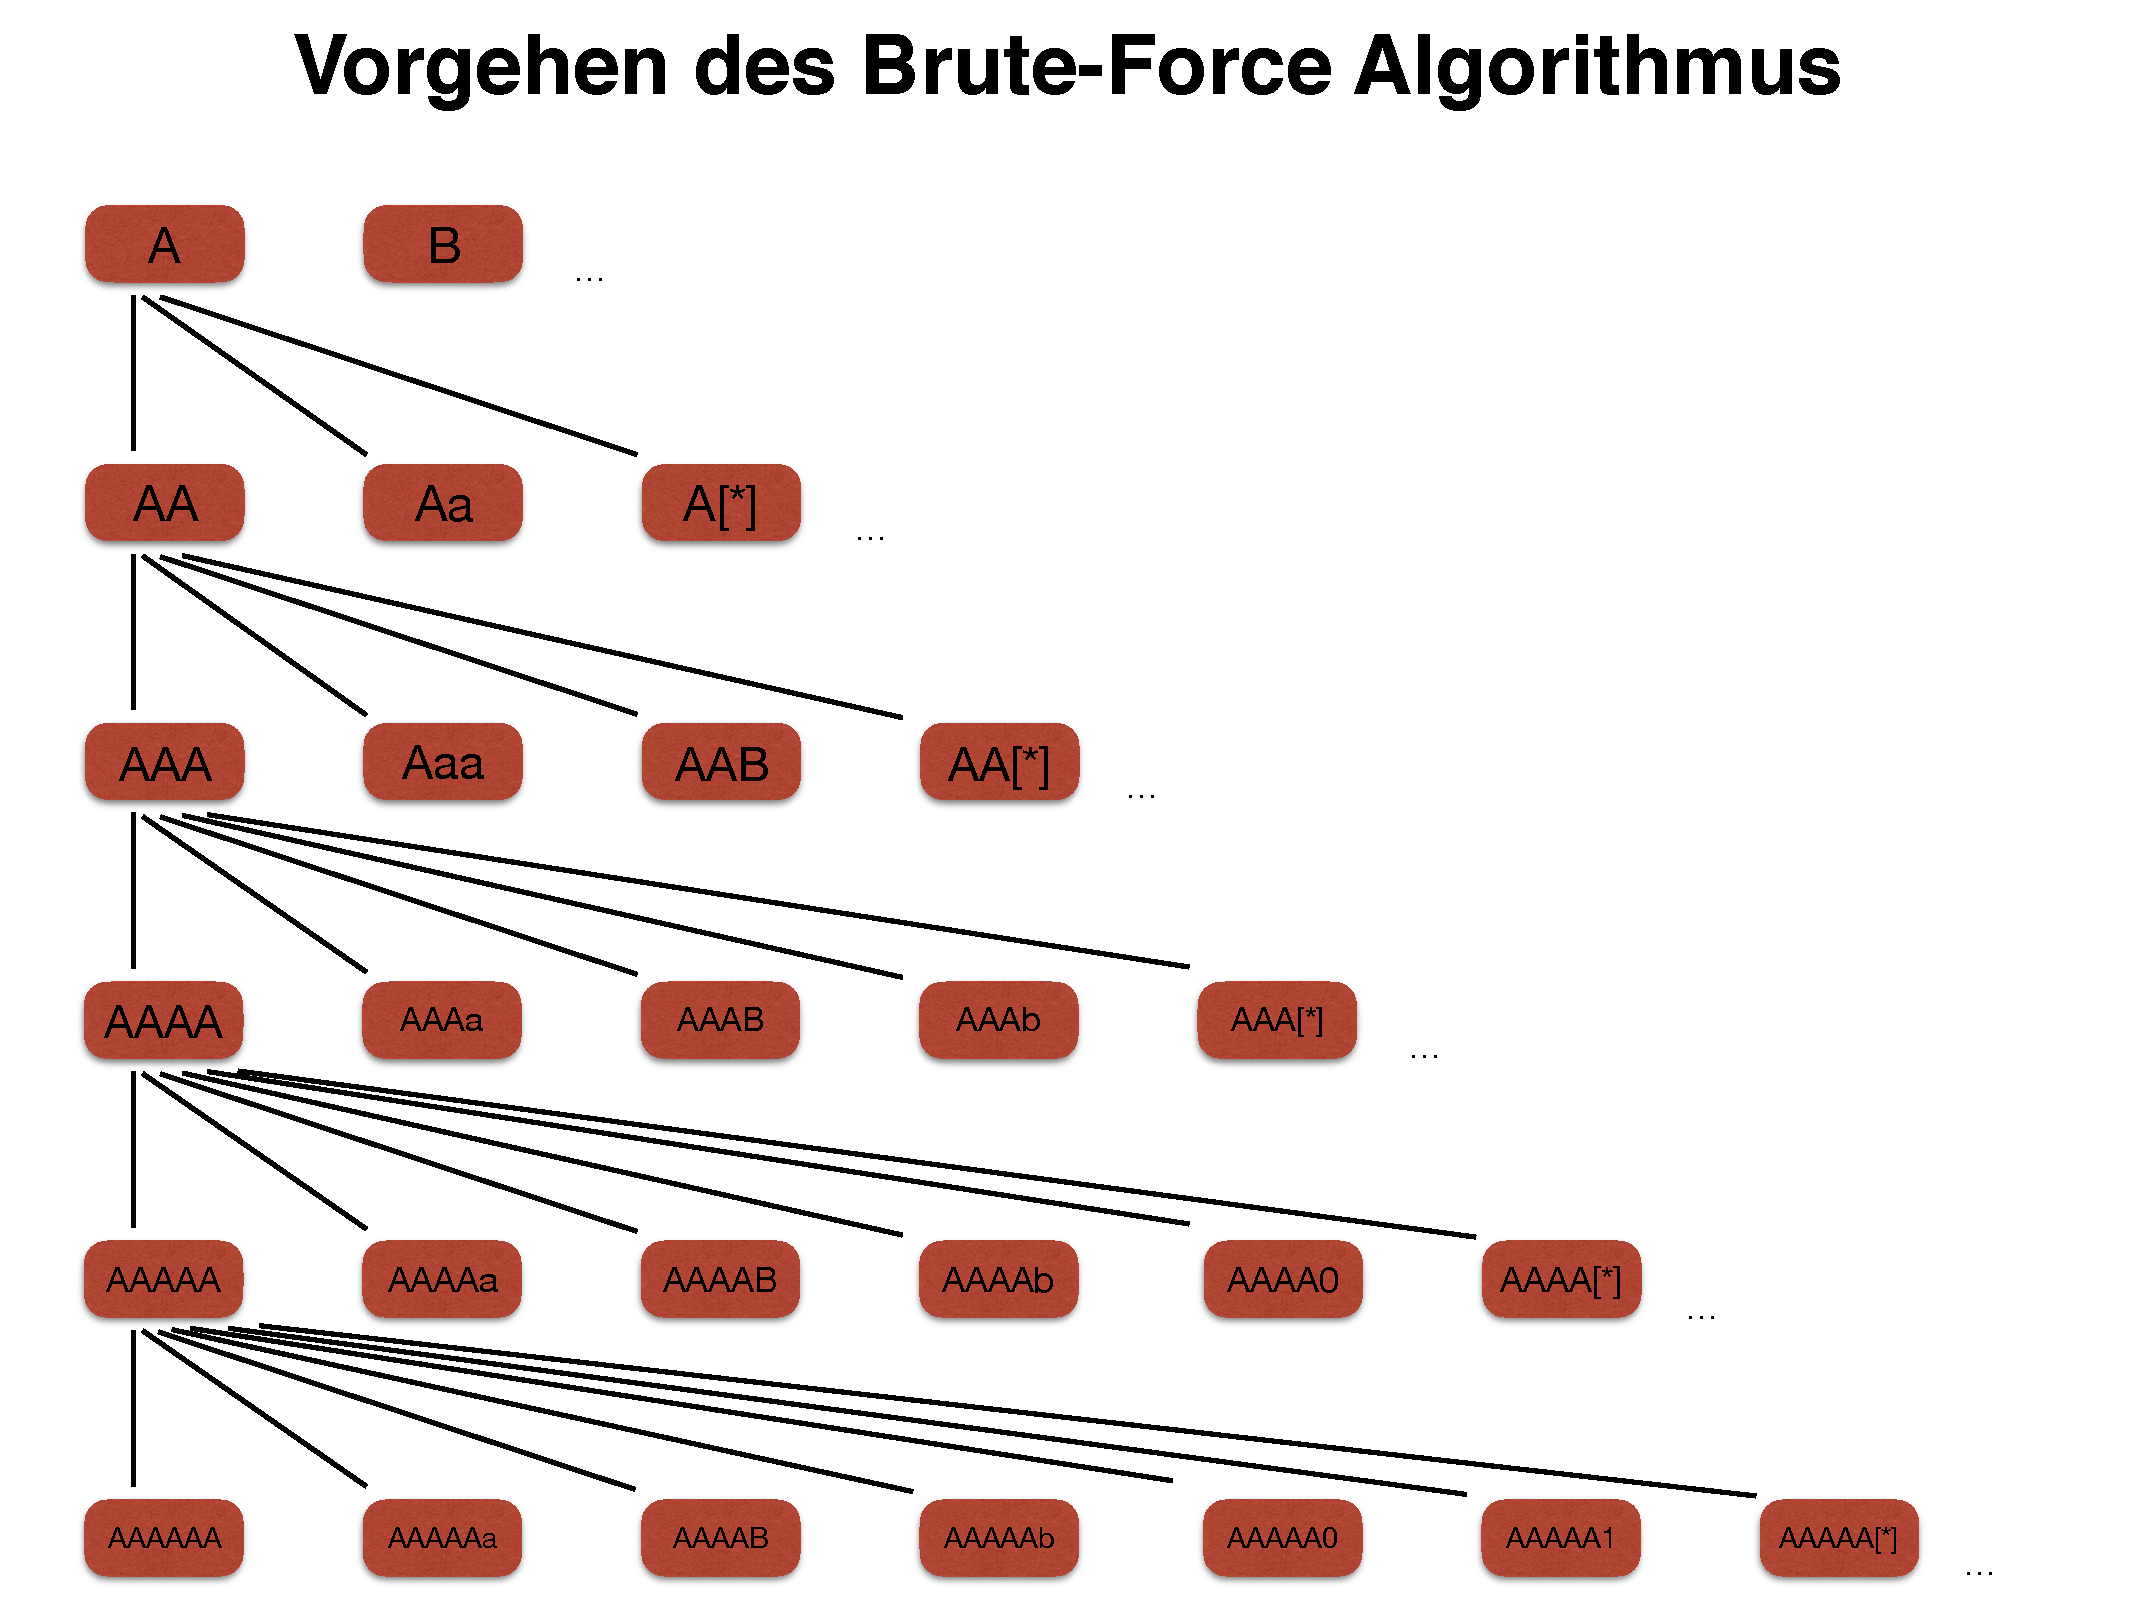
\includegraphics[natwidth=1200pt, natheight=349pt, width=1.0\textwidth]{images/SchaubildAlgorithmBreitensuche.pdf}
	\caption{Darstellung der Suchstrategie, die der Brute-Force Algorithmus zum Ermitteln des Passwortes benutzt.}
	\label{fig:showcase}
\end{figure}

%Hier Breitensuche einfügen

\section{Benutzeroberfläche}

Um Rückschlüsse auf die Geschwindigkeit verschiedener Hash-Algorithmen schließen zu können, kann bei Start der Applikation zwischen verschiedenen Hash-Algorithmen gewählt werden. Zur Auswahl stehen die Hash-Algorithmen \emph{MD5}, \emph{SHA 128} sowie \emph{SHA 256}. Die Geschwindigkeitsunterschiede beruhen primär auf der unterschiedlichen Schlüssellänge der jeweiligen Algorithmen.

\begin{figure}[!ht]
	\centering
		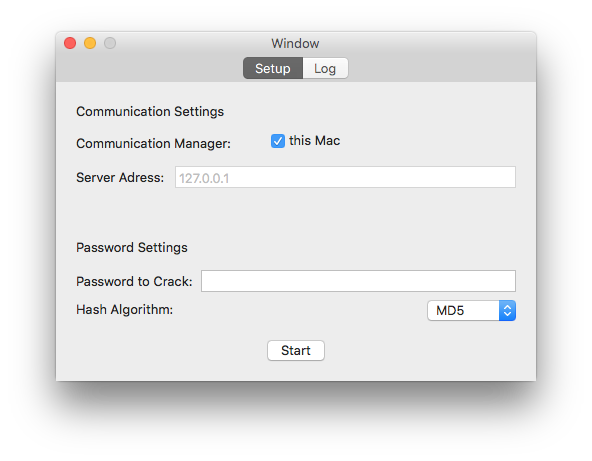
\includegraphics[natwidth=1200pt, natheight=349pt, width=0.6\textwidth]{images/WindowMaster.png}
		\caption{Benutzeroberfläche der implementierten Anwendung als Master der verteilten Anwendung}
	\label{fig:WindowMaster}
\end{figure}



\begin{figure}[!ht]
	\centering
		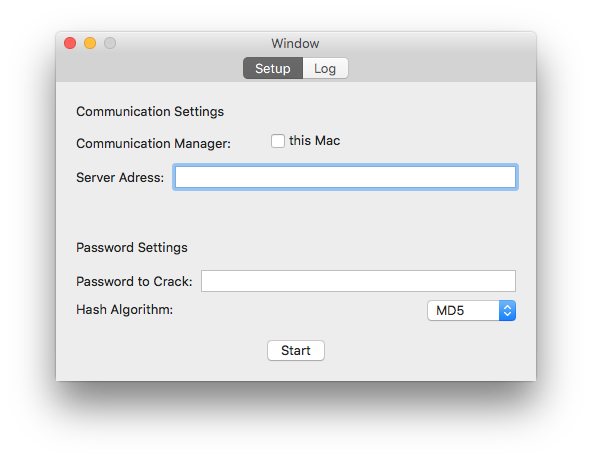
\includegraphics[natwidth=1200pt, natheight=349pt, width=0.6\textwidth]{images/WindowWorker.png}
		\caption{Benutzeroberfläche der implementierten Anwendung als Worker der verteilten Anwendung}
	\label{fig:WindowMaster}
\end{figure}


